Understanding and predicting survey performance includes modeling the likely input telemetry, the expected performance of the telescope and observatory, as well as understanding the survey strategy and its interaction with science outcomes. At this point in commissioning, the operations of the observatory are focused on obtaining specific observations, with very different strategies than will be employed during operations.  However, we can begin to evaluate how our models may be validated or not by the currently acquired observations. The science observations acquired as part of BLOCK-320  and PP-SURVEY provide the most useful visits for evaluating survey performance. 

In this section, information about zeropoints, sky background, and measured image quality (PSF size) is gathered from the ConsDb, where these values are populated by Rapid Anaysis running on the summit. These values are only populated for ACQ or OBJECT images where existing calibration data is available. We also use the bad visit list maintained by DM (the \texttt{excluded\_visits} repo) to remove on the order of 100 visits which are marked as clearly bad -- typically due to trails. This leaves us with 5008 visits from the ComCam commissioning period; 1670 of these are part of BLOCK-320 and 1848 belong to either BLOCK-320 or its precursor PP-SURVEY.

\subsubsection{Predicted throughputs and zeropoints}

The throughput curves available in \texttt{syseng\_throughputs}, the repository that tracks current system engineering summaries of full-focal-plane throughputs, can be used to predict zeropoints for average ITL CCDs. See \url{https://github.com/lsst-pst/syseng\_throughputs/blob/main/notebooks/InterpolateZeropoint.ipynb}, where a simple interpolation function for filter and airmass is defined for the current throughputs (v1.9).  Looking at only the science program visits (BLOCK-320 and PP-SURVEY), where images could be expected to be in the best possible focus and obtained under more controlled sky conditions (and where all images have 30 second exposures), we can compare the predicted 30s zeropoints to the reported median visit zeropoints in the ConsDB (the column \texttt{visit1\_quicklook.zero\_point\_median}), as shown in \figRef{zeropoints}. It is worth noting that the $u$ band is a significant outlier in this comparison of predicted versus measured zeropoint; we believe this is the same issue as discussed in \secRef{absolutethroughputs}, so is the result of either an issue in the synthetically-derived reference catalog generated for zeropoint calibration or a true underestimate of the system performance in $u$ band.  We find that the estimated zeropoints are fairly close to the achieved zeropoints, except in u band. The median offsets for the photometric nights (nights with scatter < 0.3 magnitudes; this is all science program nights except 20241126, 20241209 and 20241210) in the science survey visits are:  u = -0.26, g = 0.14, r = 0.09, i = 0.10, z = 0.13, y = 0.18. 

We applied these offsets as corrections to the zeropoints for all visits, and after also adjusting the measured zeropoints for the exposure time, can  then compare 1 second predicted and adjusted zeropoints for all visits, as in \figRef{all_zeropoints}.  As an example of a non-photometric night, see also the visits from dayObs 20241210 shown in \figRef{zeropoints_dayobs_20241210}. 

\begin{figure}
    \centering
    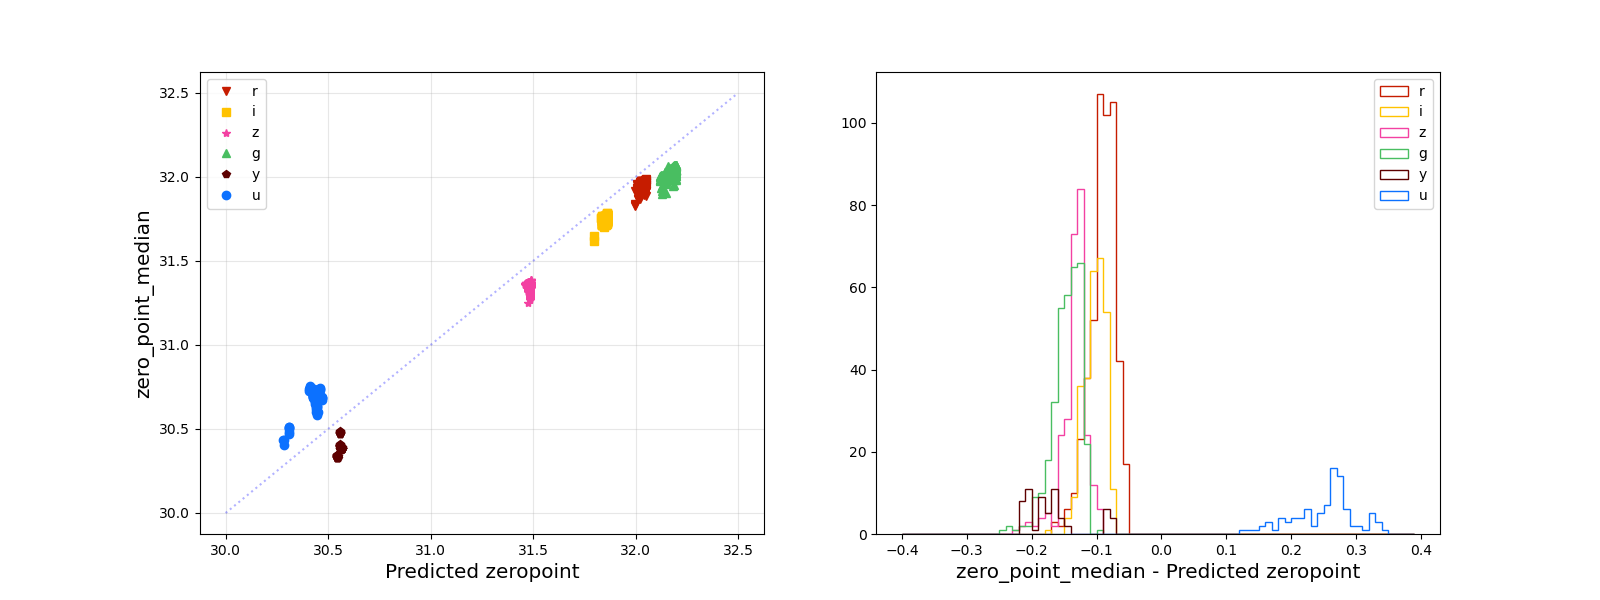
\includegraphics[width=0.8\textwidth]{sp/zeropoints.png}
    \caption{Predicted zeropoints from syseng\_throughputs (accounting for airmass) compared to measured zeropoints from \texttt{cdb\_lsst.comcam.visits1\_quicklook},  for BLOCK-320 and PP-SURVEY visits, excluding dayObs 20241126, 20241209 and  20241210. The offsets between predicted and measured zeropoints seen here can be used as a quick approximation for an updated zeropoint and applied to all visits.}
    \label{fig:zeropoints}
    \end{figure}

\begin{figure}
    \centering
    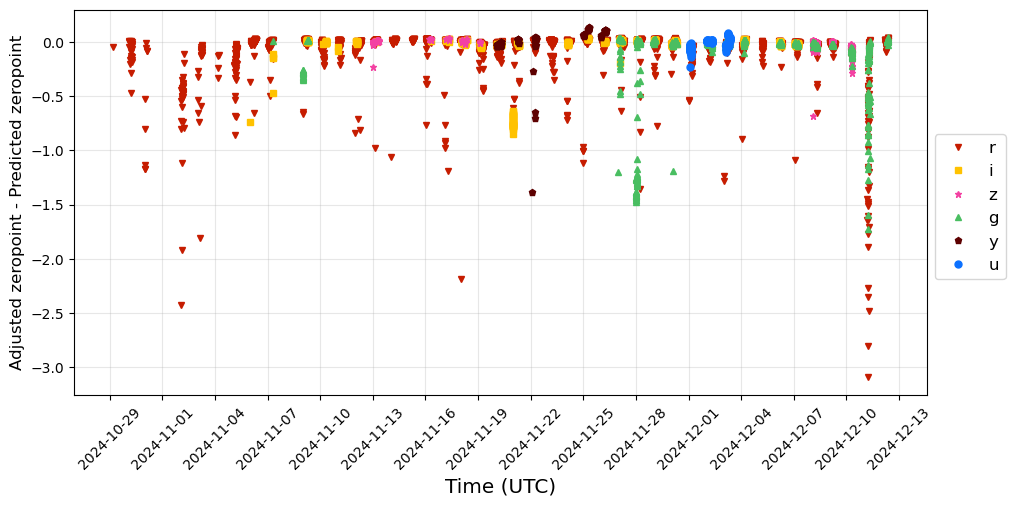
\includegraphics[width=0.7\textwidth]{sp/all_zeropoints.png}
    \caption{Measured zeropoints from \texttt{cdb\_lsst.comcam.visits1\_quicklook} adjusted for exposure time (\texttt{cdb\_lsst.comcam.visits1.shut\_time}) and our zeropoint offset, minus the predicted 1 second zeropoints from syseng\_throughputs (accounting for airmass), for all visits where the zeropoint information was reported. The offsets here are may be indicative of transparency variations, but can also indicate other potential issues such as excessively out of focus images - many of the bad images on DM's list of excluded images were also identifiable as zeropoint outliers.}
    \label{fig:all_zeropoints}
    \end{figure}


\begin{figure}
    \centering
    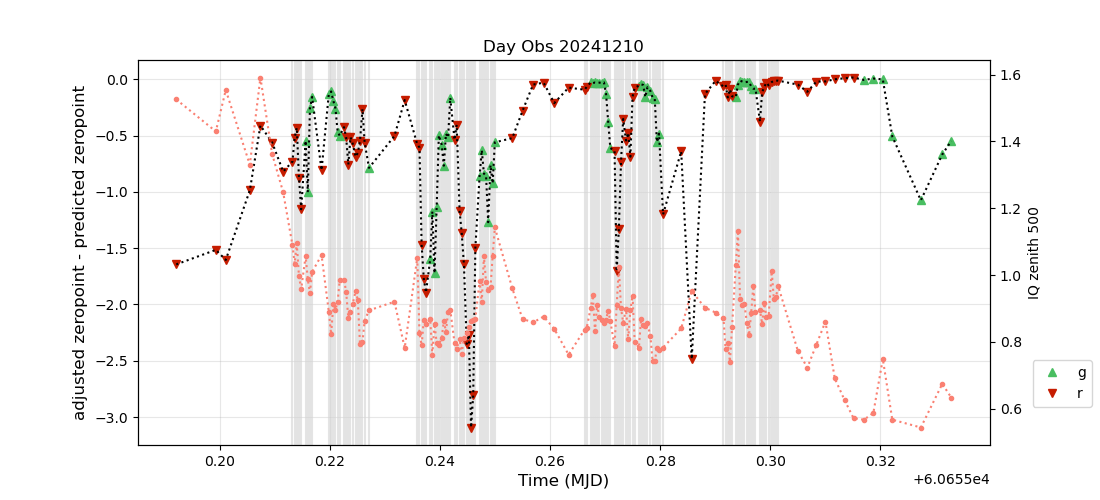
\includegraphics[width=0.7\textwidth]{sp/zeropoints_dayobs_20241210.png}
    \caption{Measured zeropoints from \texttt{cdb\_lsst.comcam.visits1\_quicklook} adjusted for exposure time (\texttt{cdb\_lsst.comcam.visits1.shut\_time}) and our zeropoint offset, minus the predicted 1 second zeropoints from syseng\_throughputs (accounting for airmass), for all ACQ and OBJECT visits on dayObs 20241210. The green upward triangles represent $g$ band while the red downward traingles represent $r$ band. The salmon dots indicate an extrapolated atmospheric seeing component, based on the \texttt{cdb\_lsst.comcam.visits1\_quicklook.psf\_sigma\_median} values adjusted to atmospheric seeing contribution at zenith, 500 nm. The gray lines indicate visits that were part of BLOCK-320. }
    \label{fig:zeropoints_dayobs_20241210}
    \end{figure}


\subsubsection{Predicted sky background}

Likewise, the survey simulations use a sky background model as part of predicting five sigma visit depths and to choose observation pointings. The outputs available in the ConsDb include a \texttt{sky\_bg\_median} value, which is in counts per pixel. Together with an estimate of the plate scale (0.2"/pixel) and the zeropoint from the hardware-only (removing atmospheric extinction), we can convert this into magnitudes per square arcsecond, to compare to the predicted values from the rubin\_scheduler sky brightness model. The results are shown in \figRef{sky}, using the measured zeropoints with offsets defined above, corrected for atmospheric extinction using coefficients determined from the \texttt{syseng\_throughputs} curves. The measured values are very consistent with the model values for the nights excluding 20241210, with a scatter of less than 0.25 magnitudes in all bands. This is within our expected errors in the sky background model, particularly in y band where the sky is quite variable and harder to model.

\begin{figure}
    \centering
    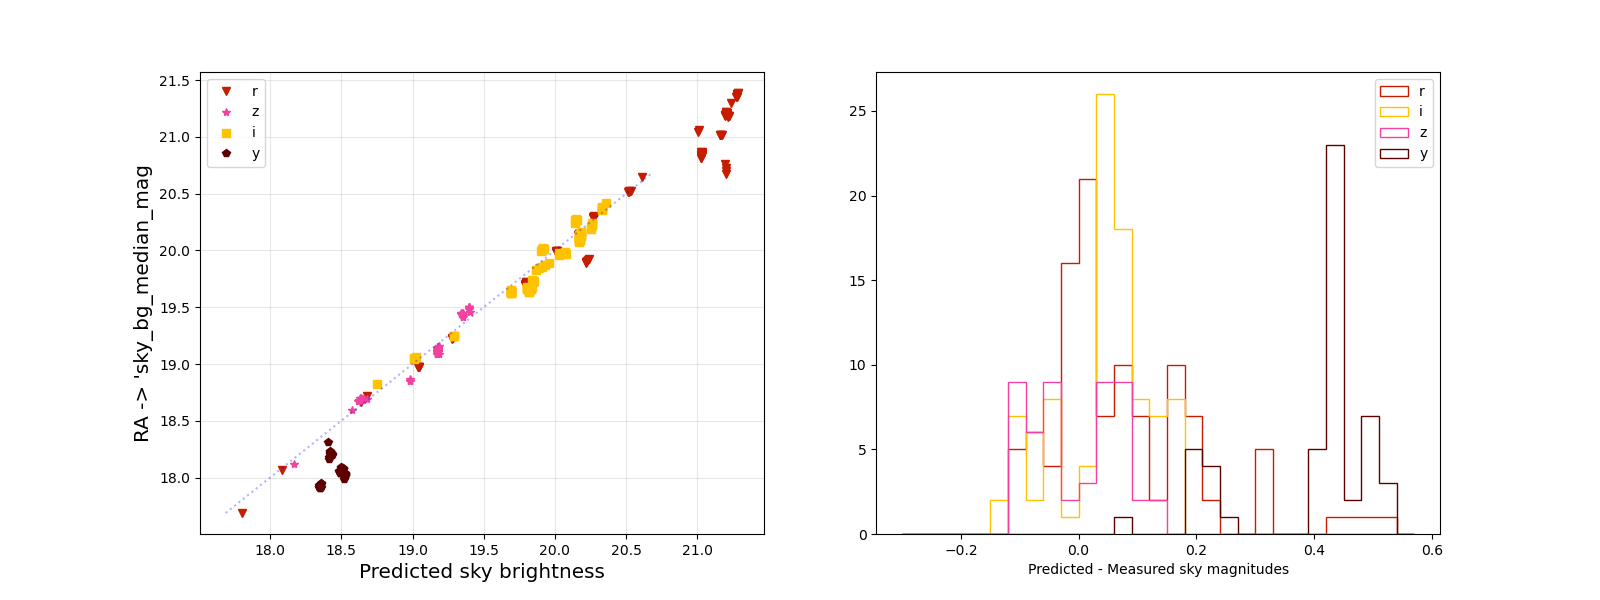
\includegraphics[width=0.8\textwidth]{sp/sky.png}
    \caption{Predicted skybrightness values from \texttt{rubin\_sim.skybrightness} compared to
      \texttt{sky\_bg\_median} converted to mags per sq arcsecond  using the adjusted zeropoints based on the values in  \texttt{visits1\_quicklook.zero\_point\_median}.}
    \label{fig:sky}
    \end{figure}


\subsubsection{Predicted seeing}

We look forward to comparing seeing performance to survey predictions as more information is available about the system contribution and atmosphere state via a Rubin DIMM. Initial estimates indicate that the approximate equivalent of seeingFwhmGeom for the science program visits had a mean of around 1 arcsecond, which is very close to average long-term survey expectations, where the mean value is around 0.9 arcseconds. This is particularly impressive for this early phase of commissioning. 

\begin{figure}
    \centering
    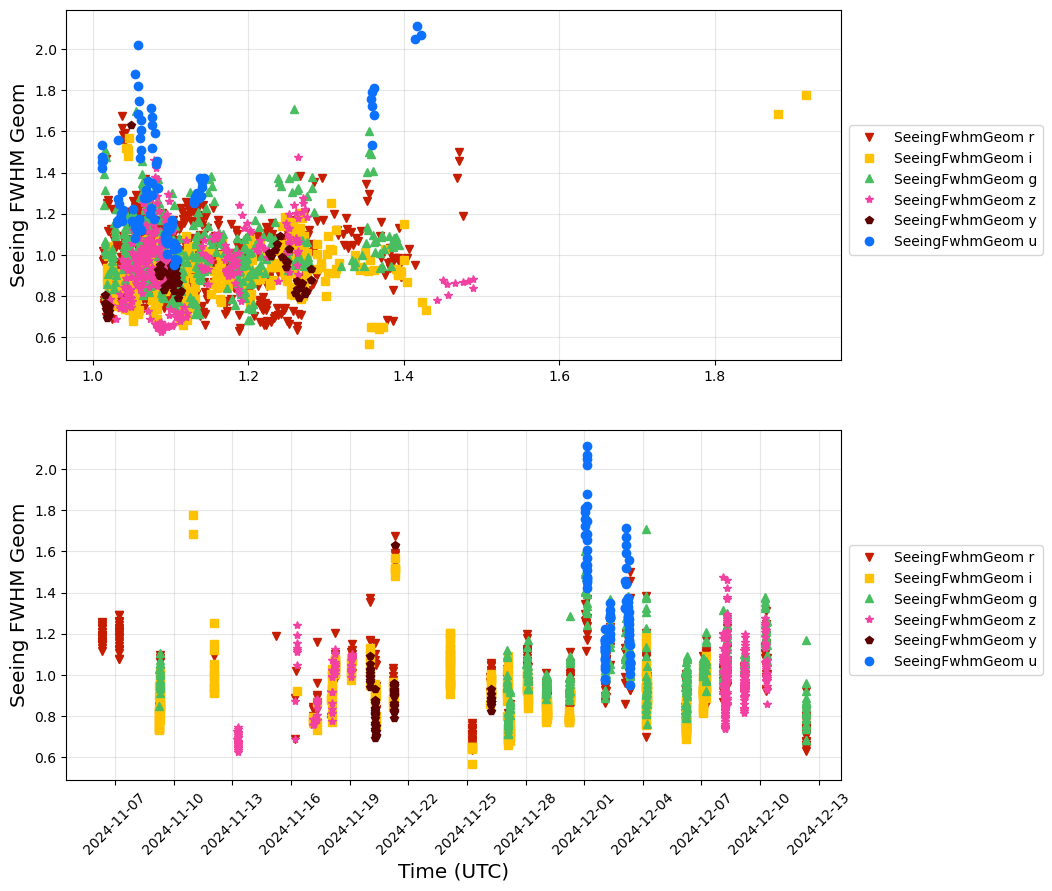
\includegraphics[width=0.7\textwidth]{sp/seeing.png}
    \caption{Values of \texttt{psf\_sigma\_median} are converted into \texttt{seeingFwhmGeom} as determined from OR4 simulations. The mean \texttt{seeingFwhmGeom} in simulations is around 0.9 arcseconds, close to the 1.0 arcsecond mean value in these visits.}
    \label{fig:seeing}
    \end{figure}


\subsubsection{Slew times}

As part of the process of commissioning, the movement of the TMA was ramped up from an initial  1\% of potential velocity/acceleration/jerk performance, with additional settle times built into various components, to 20\% of TMA maximum velocity/acceleration/jerk and greatly reduced settle and wait times. In programs such as the AOS triplets, there are additional movements that must be performed with the telescope, such as moving the focal plane to adjust focus and applying bending modes to the mirror, so here we look at the visits acquired as part of BLOCK-320. These visits included small dither offsets on the order of 0.2 degrees or so for all fields except Rubin\_SV\_095\_-25 which had a slightly larger dither pattern. 

The decrease in time between visits in BLOCK-320 (and corresponding increase in survey efficiency) is shown in \figRef{time_between_visits}.  Within each night, the median time between observations is indicated, along with a breakdown of the time spent actively moving the TMA ("TMA slew") and the time spent in settle or waiting for ready reports from various components ("wait before TMA slew" and "wait after TMA slew"). As these are very small slews, the increase in TMA velocity from 1\% to 20\% did result in an improvement of about 1 second, however this was minor in comparison to the reduction in wait and settle times. Some of the wait after slew can be linked to filter changes, although typically the number of filter changes is few enough to be missed by the median. The bulk of the wait and settles before and after the TMA slew was slowly whittled away over the course of commissioning. In the last few days of comcam observing, the wait time after the shutter closed and before the TMA started moving was reduced to 1 second. The settle time after TMA movement was reduced to zero. 

Survey simulations have assumed we would need a 3 second settle after TMA movement. If image quality indicates that this additional settle time is unnecessary, even as the TMA velocities are increased, this could provide a significant bonus to overall survey efficiency by reducing the time between visits from a typical 5 seconds to something potentially as small as 2.5 seconds.

%On dayObs 20241211, an AOS block was performed using a pointing pattern similar to what we might find with the main survey - offsets between pointings were on the order of the LSSTCam field of view. This program, BLOCK-T345, had significant additional overheads in each visit including pistoning the focal plane to intra- and extra- focus positions, which make it difficult to directly compare the time between visits to what we might expect from true survey operations. However, we can look at the TMA slew movement and compare to  the slew time expected from a model configured similarly to the Simonyi Telescope. We find that the model slew predictions match the TMA slew events within 1 second.  

\begin{figure}
    \centering
    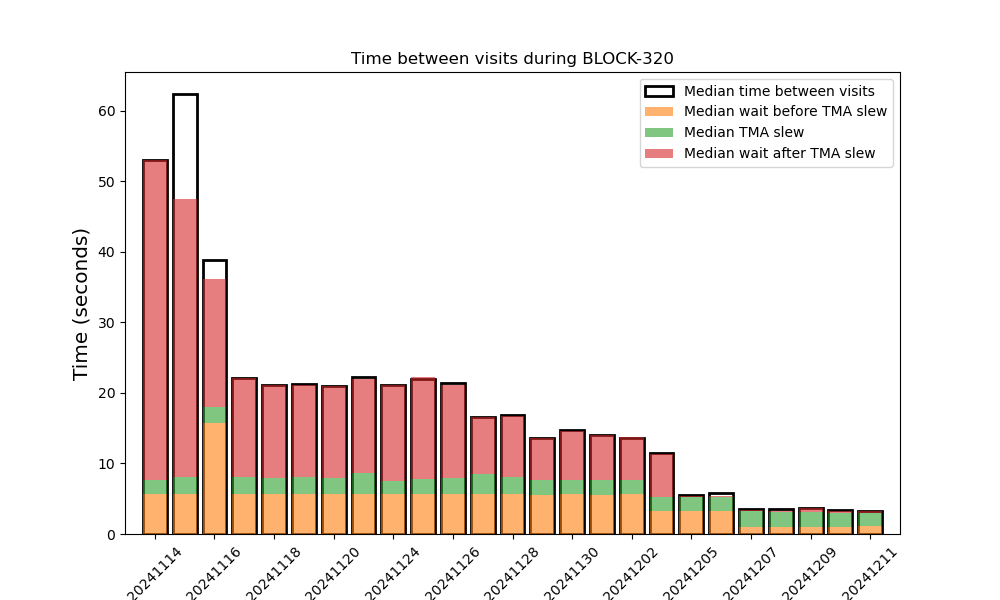
\includegraphics[width=0.8\textwidth]{sp/TimeBetweenVisits.png}
    \caption{Time between successive visits for Science Pipelines commissioning observations in BLOCK-320. The median time between visits is outlined in black. The median time of active TMA slewing is indicated in green. These active TMA slews are typically sandwiched by a short settle or wait time before moving, and another wait or settle after movement. The wait before slew is indicated in orange, while the wait after the slew is indicated in red. Places where the median of these separate events is less than the total median time between slews generally corresponds to a sequence which contained a fault, usually combined with a number of other slightly longer-than-usual events such as filter changes. The filter changes increase the wait time after TMA movement, but not quite frequently enough to impact the median; the fault increases the total time between visits for a single slew, and this happens to push the median time between visits into one of the slightly longer than typical slews (and perhaps even into one of the filter change slews). }
    \label{fig:time_between_visits}
    \end{figure}


Remaining questions relevant to survey strategy include the efficiency of observations, both sequential observations with standard slew offsets and sustained over many hours and days, and the likelihood of whether a single exposure per visit will be sufficient.

%\begin{figure}
%  \centering
%     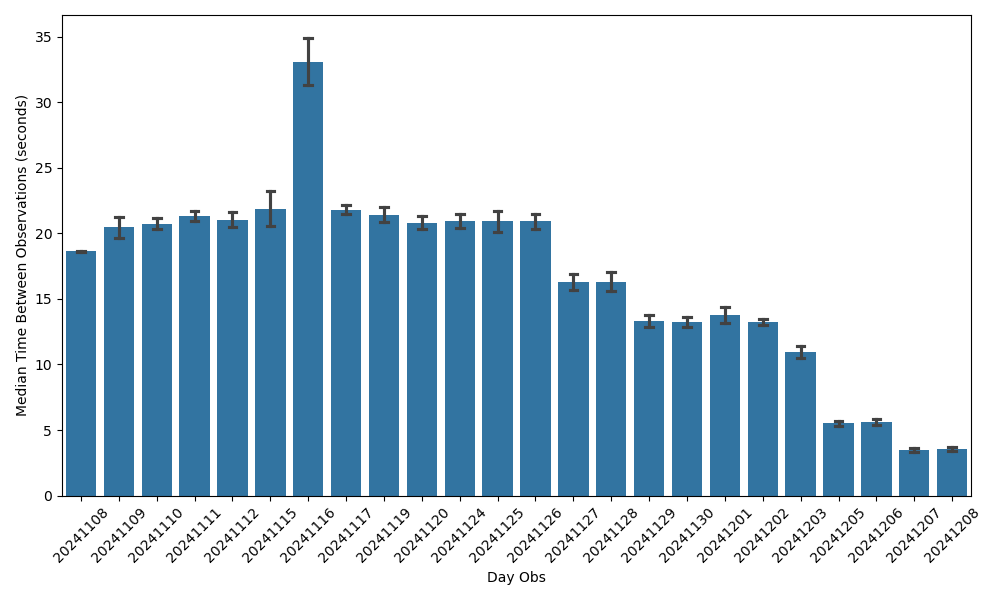
\includegraphics[width=0.7\textwidth]{sp/timeBetweenExposures20241208.png}
%    \caption{Time between successive visits for Science Pipelines commissioning observations.}
%    \label{fig:time_between_visits}
% \end{figure}